\chapter{图的遍历}

本章讨论两种基本的图算法：深度优先搜索和广度优先搜索。两种算法都从图中的一个起始节点出发，访问从该节点能够到达的所有节点。它们的区别在于访问节点的顺序。

\section{深度优先搜索}

\index{depth-first search}

\key{深度优先搜索}（DFS）是一种直接的图遍历方法。算法从起始节点开始，沿图中的边前往从该节点能够到达的所有其他节点。

只要还能发现新节点，深度优先搜索就会沿图中的一条路径不断前进。随后，它返回先前的节点并开始探索图的其他部分。算法会记录已经访问过的节点，从而保证每个节点只处理一次。

\subsubsection*{示例}

考察深度优先搜索如何处理下图：
\begin{center}
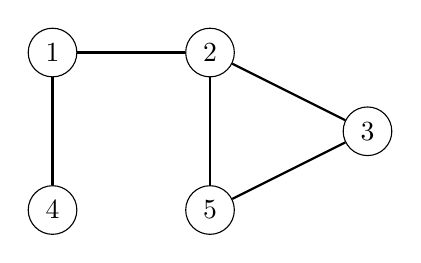
\begin{tikzpicture}
\node[draw, circle] (1) at (1,5) {$1$};
\node[draw, circle] (2) at (3,5) {$2$};
\node[draw, circle] (3) at (5,4) {$3$};
\node[draw, circle] (4) at (1,3) {$4$};
\node[draw, circle] (5) at (3,3) {$5$};

\path[draw,thick,-] (1) -- (2);
\path[draw,thick,-] (2) -- (3);
\path[draw,thick,-] (1) -- (4);
\path[draw,thick,-] (3) -- (5);
\path[draw,thick,-] (2) -- (5);
\end{tikzpicture}
\end{center}
搜索可以从图中任意节点开始；这里从节点 1 开始。

搜索首先前往节点 2：
\begin{center}
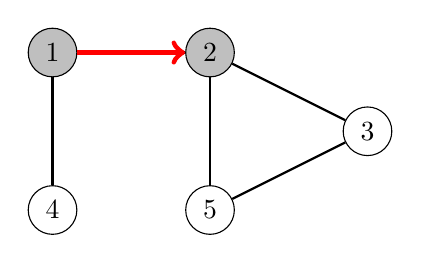
\begin{tikzpicture}
\node[draw, circle,fill=lightgray] (1) at (1,5) {$1$};
\node[draw, circle,fill=lightgray] (2) at (3,5) {$2$};
\node[draw, circle] (3) at (5,4) {$3$};
\node[draw, circle] (4) at (1,3) {$4$};
\node[draw, circle] (5) at (3,3) {$5$};

\path[draw,thick,-] (1) -- (2);
\path[draw,thick,-] (2) -- (3);
\path[draw,thick,-] (1) -- (4);
\path[draw,thick,-] (3) -- (5);
\path[draw,thick,-] (2) -- (5);

\path[draw=red,thick,->,line width=2pt] (1) -- (2);
\end{tikzpicture}
\end{center}
随后访问节点 3 和 5：
\begin{center}
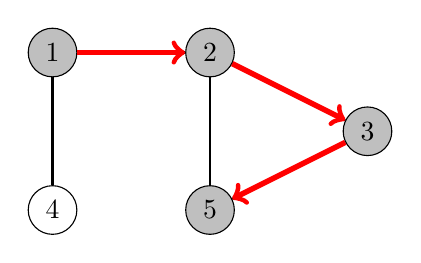
\begin{tikzpicture}
\node[draw, circle,fill=lightgray] (1) at (1,5) {$1$};
\node[draw, circle,fill=lightgray] (2) at (3,5) {$2$};
\node[draw, circle,fill=lightgray] (3) at (5,4) {$3$};
\node[draw, circle] (4) at (1,3) {$4$};
\node[draw, circle,fill=lightgray] (5) at (3,3) {$5$};

\path[draw,thick,-] (1) -- (2);
\path[draw,thick,-] (2) -- (3);
\path[draw,thick,-] (1) -- (4);
\path[draw,thick,-] (3) -- (5);
\path[draw,thick,-] (2) -- (5);

\path[draw=red,thick,->,line width=2pt] (1) -- (2);
\path[draw=red,thick,->,line width=2pt] (2) -- (3);
\path[draw=red,thick,->,line width=2pt] (3) -- (5);
\end{tikzpicture}
\end{center}
节点 5 的邻居是 2 和 3，但搜索已经访问过二者，因此现在要返回先前的节点。节点 3 和 2 的邻居也都已访问，所以下一步从节点 1 前往节点 4：
\begin{center}
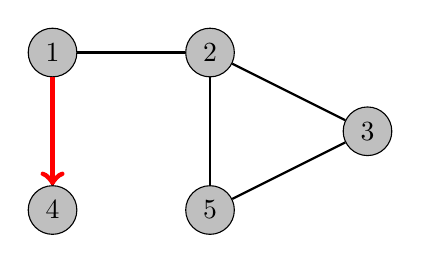
\begin{tikzpicture}
\node[draw, circle,fill=lightgray] (1) at (1,5) {$1$};
\node[draw, circle,fill=lightgray] (2) at (3,5) {$2$};
\node[draw, circle,fill=lightgray] (3) at (5,4) {$3$};
\node[draw, circle,fill=lightgray] (4) at (1,3) {$4$};
\node[draw, circle,fill=lightgray] (5) at (3,3) {$5$};

\path[draw,thick,-] (1) -- (2);
\path[draw,thick,-] (2) -- (3);
\path[draw,thick,-] (1) -- (4);
\path[draw,thick,-] (3) -- (5);
\path[draw,thick,-] (2) -- (5);

\path[draw=red,thick,->,line width=2pt] (1) -- (4);
\end{tikzpicture}
\end{center}
至此所有节点都已访问，搜索结束。

深度优先搜索的时间复杂度为 $O(n+m)$，其中 $n$ 为节点数，$m$ 为边数，因为算法会把每个节点和每条边处理一次。

\subsubsection*{实现}

使用递归可以很方便地实现深度优先搜索。下面的函数 \texttt{dfs} 从给定节点开始深度优先搜索。函数假定图以邻接表形式存储在数组
\begin{lstlisting}
vector<int> adj[N];
\end{lstlisting}
中，并维护数组
\begin{lstlisting}
bool visited[N];
\end{lstlisting}
来记录已经访问的节点。初始时数组中每个值都是 \texttt{false}；搜索到达节点 $s$ 时，\texttt{visited}[$s$] 变为 \texttt{true}。函数可实现如下：
\begin{lstlisting}
void dfs(int s) {
    if (visited[s]) return;
    visited[s] = true;
    // process node s
    for (auto u: adj[s]) {
        dfs(u);
    }
}
\end{lstlisting}

\section{广度优先搜索}

\index{breadth-first search}

\key{广度优先搜索}（BFS）按照与起始节点的距离从小到大访问节点。因此，我们可以用广度优先搜索计算起始节点到所有其他节点的距离。不过，广度优先搜索的实现比深度优先搜索更复杂。

广度优先搜索逐层遍历节点。搜索首先探索与起始节点距离为 1 的节点，然后探索距离为 2 的节点，依此类推，直到所有节点均已访问。

\subsubsection*{示例}

考察广度优先搜索如何处理下图：

\begin{center}
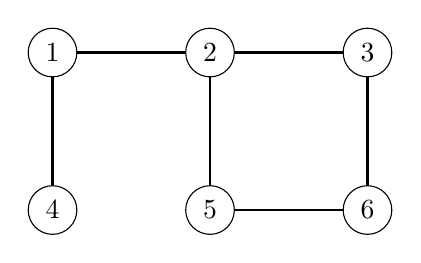
\begin{tikzpicture}
\node[draw, circle] (1) at (1,5) {$1$};
\node[draw, circle] (2) at (3,5) {$2$};
\node[draw, circle] (3) at (5,5) {$3$};
\node[draw, circle] (4) at (1,3) {$4$};
\node[draw, circle] (5) at (3,3) {$5$};
\node[draw, circle] (6) at (5,3) {$6$};

\path[draw,thick,-] (1) -- (2);
\path[draw,thick,-] (2) -- (3);
\path[draw,thick,-] (1) -- (4);
\path[draw,thick,-] (3) -- (6);
\path[draw,thick,-] (2) -- (5);
\path[draw,thick,-] (5) -- (6);
\end{tikzpicture}
\end{center}
假设搜索从节点 1 开始。首先处理从节点 1 经过一条边即可到达的所有节点：
\begin{center}
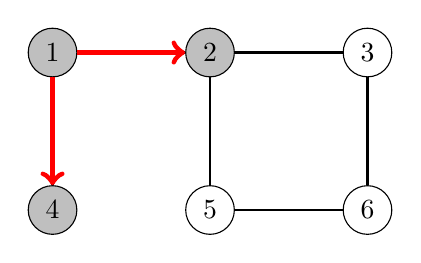
\begin{tikzpicture}
\node[draw, circle,fill=lightgray] (1) at (1,5) {$1$};
\node[draw, circle,fill=lightgray] (2) at (3,5) {$2$};
\node[draw, circle] (3) at (5,5) {$3$};
\node[draw, circle,fill=lightgray] (4) at (1,3) {$4$};
\node[draw, circle] (5) at (3,3) {$5$};
\node[draw, circle] (6) at (5,3) {$6$};

\path[draw,thick,-] (1) -- (2);
\path[draw,thick,-] (2) -- (3);
\path[draw,thick,-] (1) -- (4);
\path[draw,thick,-] (3) -- (6);
\path[draw,thick,-] (2) -- (5);
\path[draw,thick,-] (5) -- (6);

\path[draw,thick,-] (1) -- (2);
\path[draw,thick,-] (2) -- (3);
\path[draw,thick,-] (1) -- (4);
\path[draw,thick,-] (2) -- (5);

\path[draw=red,thick,->,line width=2pt] (1) -- (2);
\path[draw=red,thick,->,line width=2pt] (1) -- (4);
\end{tikzpicture}
\end{center}
随后前往节点 3 和 5：
\begin{center}
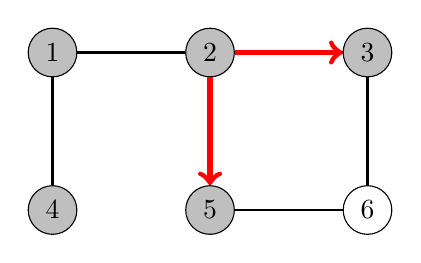
\begin{tikzpicture}
\node[draw, circle,fill=lightgray] (1) at (1,5) {$1$};
\node[draw, circle,fill=lightgray] (2) at (3,5) {$2$};
\node[draw, circle,fill=lightgray] (3) at (5,5) {$3$};
\node[draw, circle,fill=lightgray] (4) at (1,3) {$4$};
\node[draw, circle,fill=lightgray] (5) at (3,3) {$5$};
\node[draw, circle] (6) at (5,3) {$6$};

\path[draw,thick,-] (1) -- (2);
\path[draw,thick,-] (2) -- (3);
\path[draw,thick,-] (1) -- (4);
\path[draw,thick,-] (3) -- (6);
\path[draw,thick,-] (2) -- (5);
\path[draw,thick,-] (5) -- (6);

\path[draw,thick,-] (1) -- (2);
\path[draw,thick,-] (2) -- (3);
\path[draw,thick,-] (1) -- (4);
\path[draw,thick,-] (2) -- (5);

\path[draw=red,thick,->,line width=2pt] (2) -- (3);
\path[draw=red,thick,->,line width=2pt] (2) -- (5);
\end{tikzpicture}
\end{center}
最后访问节点 6：
\begin{center}
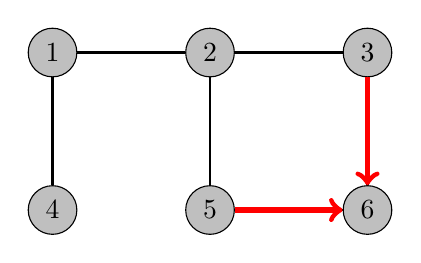
\begin{tikzpicture}
\node[draw, circle,fill=lightgray] (1) at (1,5) {$1$};
\node[draw, circle,fill=lightgray] (2) at (3,5) {$2$};
\node[draw, circle,fill=lightgray] (3) at (5,5) {$3$};
\node[draw, circle,fill=lightgray] (4) at (1,3) {$4$};
\node[draw, circle,fill=lightgray] (5) at (3,3) {$5$};
\node[draw, circle,fill=lightgray] (6) at (5,3) {$6$};

\path[draw,thick,-] (1) -- (2);
\path[draw,thick,-] (2) -- (3);
\path[draw,thick,-] (1) -- (4);
\path[draw,thick,-] (3) -- (6);
\path[draw,thick,-] (2) -- (5);
\path[draw,thick,-] (5) -- (6);

\path[draw,thick,-] (1) -- (2);
\path[draw,thick,-] (2) -- (3);
\path[draw,thick,-] (1) -- (4);
\path[draw,thick,-] (2) -- (5);

\path[draw=red,thick,->,line width=2pt] (3) -- (6);
\path[draw=red,thick,->,line width=2pt] (5) -- (6);
\end{tikzpicture}
\end{center}
现在已经算出起始节点到图中所有节点的距离：

\begin{tabular}{ll}
\\
节点 & 距离 \\
\hline
1 & 0 \\
2 & 1 \\
3 & 2 \\
4 & 1 \\
5 & 2 \\
6 & 3 \\
\\
\end{tabular}

与深度优先搜索一样，广度优先搜索的时间复杂度也是 $O(n+m)$，其中 $n$ 为节点数，$m$ 为边数。

\subsubsection*{实现}

广度优先搜索的实现比深度优先搜索更复杂，因为算法会访问图中不同区域的节点。典型实现基于一个存放节点的队列；每一步处理队首的下一个节点。

以下代码假定图以邻接表存储，并维护这些数据结构：
\begin{lstlisting}
queue<int> q;
bool visited[N];
int distance[N];
\end{lstlisting}

队列 \texttt{q} 按距离递增的顺序保存待处理节点。新节点总是加入队尾，而队首节点是下一个待处理节点。数组 \texttt{visited} 表示搜索已经访问了哪些节点，数组 \texttt{distance} 则保存起始节点到图中所有节点的距离。

从节点 $x$ 开始的搜索可实现如下：
\begin{lstlisting}
visited[x] = true;
distance[x] = 0;
q.push(x);
while (!q.empty()) {
    int s = q.front(); q.pop();
    // process node s
    for (auto u : adj[s]) {
        if (visited[u]) continue;
        visited[u] = true;
        distance[u] = distance[s]+1;
        q.push(u);
    }
}
\end{lstlisting}

\section{应用}

利用图遍历算法，我们可以检查图的许多性质。通常深度优先搜索和广度优先搜索都能使用；实际中深度优先搜索往往更合适，因为它更容易实现。在以下应用中，我们假定图是无向图。

\subsubsection{连通性检查}

\index{connected graph}

若图中任意两个节点之间都存在路径，则称图是连通的。因此，从任意节点出发，检查是否能到达所有其他节点，就可以判断图是否连通。

例如，在图
\begin{center}
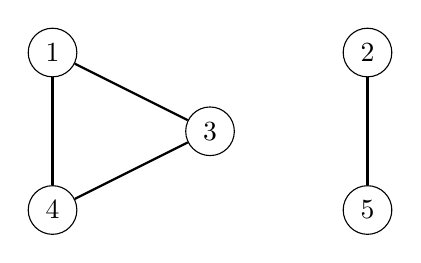
\begin{tikzpicture}
\node[draw, circle] (2) at (7,5) {$2$};
\node[draw, circle] (1) at (3,5) {$1$};
\node[draw, circle] (3) at (5,4) {$3$};
\node[draw, circle] (5) at (7,3) {$5$};
\node[draw, circle] (4) at (3,3) {$4$};

\path[draw,thick,-] (1) -- (3);
\path[draw,thick,-] (1) -- (4);
\path[draw,thick,-] (3) -- (4);
\path[draw,thick,-] (2) -- (5);
\end{tikzpicture}
\end{center}
中，从节点 $1$ 开始的深度优先搜索会访问以下节点：
\begin{center}
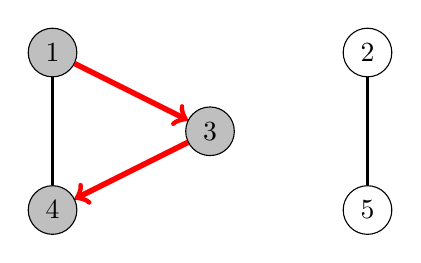
\begin{tikzpicture}
\node[draw, circle] (2) at (7,5) {$2$};
\node[draw, circle,fill=lightgray] (1) at (3,5) {$1$};
\node[draw, circle,fill=lightgray] (3) at (5,4) {$3$};
\node[draw, circle] (5) at (7,3) {$5$};
\node[draw, circle,fill=lightgray] (4) at (3,3) {$4$};

\path[draw,thick,-] (1) -- (3);
\path[draw,thick,-] (1) -- (4);
\path[draw,thick,-] (3) -- (4);
\path[draw,thick,-] (2) -- (5);

\path[draw=red,thick,->,line width=2pt] (1) -- (3);
\path[draw=red,thick,->,line width=2pt] (3) -- (4);

\end{tikzpicture}
\end{center}

由于搜索没有访问所有节点，可以断定该图不连通。类似地，遍历各个节点，每当当前节点尚不属于任何分量时就启动一次新的深度优先搜索，还可以找出图的所有连通分量。

\subsubsection{寻找环}

\index{cycle}

在图遍历过程中，如果发现某个节点的一个邻居已经访问过，并且该邻居不是当前路径上的前一个节点，那么图中就存在环。例如，图
\begin{center}
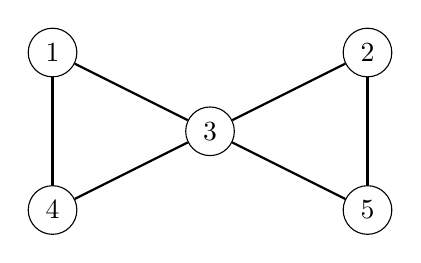
\begin{tikzpicture}
\node[draw, circle] (2) at (7,5) {$2$};
\node[draw, circle] (1) at (3,5) {$1$};
\node[draw, circle] (3) at (5,4) {$3$};
\node[draw, circle] (5) at (7,3) {$5$};
\node[draw, circle] (4) at (3,3) {$4$};

\path[draw,thick,-] (1) -- (3);
\path[draw,thick,-] (1) -- (4);
\path[draw,thick,-] (3) -- (4);
\path[draw,thick,-] (2) -- (5);
\path[draw,thick,-] (2) -- (3);
\path[draw,thick,-] (3) -- (5);
\end{tikzpicture}
\end{center}
包含两个环。可以按如下方式找到其中一个：
\begin{center}
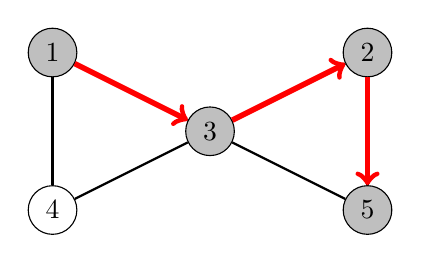
\begin{tikzpicture}
\node[draw, circle,fill=lightgray] (2) at (7,5) {$2$};
\node[draw, circle,fill=lightgray] (1) at (3,5) {$1$};
\node[draw, circle,fill=lightgray] (3) at (5,4) {$3$};
\node[draw, circle,fill=lightgray] (5) at (7,3) {$5$};
\node[draw, circle] (4) at (3,3) {$4$};

\path[draw,thick,-] (1) -- (3);
\path[draw,thick,-] (1) -- (4);
\path[draw,thick,-] (3) -- (4);
\path[draw,thick,-] (2) -- (5);
\path[draw,thick,-] (2) -- (3);
\path[draw,thick,-] (3) -- (5);

\path[draw=red,thick,->,line width=2pt] (1) -- (3);
\path[draw=red,thick,->,line width=2pt] (3) -- (2);
\path[draw=red,thick,->,line width=2pt] (2) -- (5);

\end{tikzpicture}
\end{center}
从节点 2 移动到节点 5 后，我们发现节点 5 的邻居 3 已经访问过。因此，图中存在一个经过节点 3 的环，例如 $3 \rightarrow 2 \rightarrow 5 \rightarrow 3$。

判断图中是否含环的另一种方法，是直接计算每个分量的节点数与边数。若一个分量含有 $c$ 个节点且没有环，它必须恰好含有 $c-1$ 条边（因而是一棵树）。如果边数不少于 $c$，该分量一定含环。

\subsubsection{二分图检查}

\index{bipartite graph}

如果可以用两种颜色给图中的节点着色，使任意相邻节点颜色都不同，则该图是二分图。使用图遍历算法判断一个图是否为二分图出乎意料地简单。

基本思想是把起始节点染成蓝色，把它的所有邻居染成红色，再把这些邻居的邻居染成蓝色，依此类推。如果搜索过程中发现两个相邻节点颜色相同，图就不是二分图；否则图是二分图，并且我们已经得到一种合法着色。

例如，图
\begin{center}
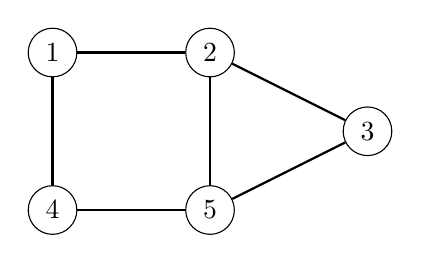
\begin{tikzpicture}
\node[draw, circle] (2) at (5,5) {$2$};
\node[draw, circle] (1) at (3,5) {$1$};
\node[draw, circle] (3) at (7,4) {$3$};
\node[draw, circle] (5) at (5,3) {$5$};
\node[draw, circle] (4) at (3,3) {$4$};

\path[draw,thick,-] (1) -- (2);
\path[draw,thick,-] (2) -- (5);
\path[draw,thick,-] (5) -- (4);
\path[draw,thick,-] (4) -- (1);
\path[draw,thick,-] (2) -- (3);
\path[draw,thick,-] (5) -- (3);
\end{tikzpicture}
\end{center}
不是二分图，因为从节点 1 开始的搜索过程如下：
\begin{center}
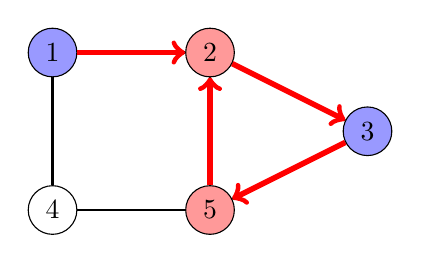
\begin{tikzpicture}
\node[draw, circle,fill=red!40] (2) at (5,5) {$2$};
\node[draw, circle,fill=blue!40] (1) at (3,5) {$1$};
\node[draw, circle,fill=blue!40] (3) at (7,4) {$3$};
\node[draw, circle,fill=red!40] (5) at (5,3) {$5$};
\node[draw, circle] (4) at (3,3) {$4$};

\path[draw,thick,-] (1) -- (2);
\path[draw,thick,-] (2) -- (5);
\path[draw,thick,-] (5) -- (4);
\path[draw,thick,-] (4) -- (1);
\path[draw,thick,-] (2) -- (3);
\path[draw,thick,-] (5) -- (3);

\path[draw=red,thick,->,line width=2pt] (1) -- (2);
\path[draw=red,thick,->,line width=2pt] (2) -- (3);
\path[draw=red,thick,->,line width=2pt] (3) -- (5);
\path[draw=red,thick,->,line width=2pt] (5) -- (2);
\end{tikzpicture}
\end{center}
可以看到，节点 2 和 5 都被染成红色，但它们在图中相邻，因此该图不是二分图。

该算法总是正确的，因为只有两种颜色可用时，一个分量中起始节点的颜色就决定了该分量内所有其他节点的颜色。起始节点染成红色还是蓝色并无影响。

需要注意，一般情况下，要判断图中节点能否使用 $k$ 种颜色着色、同时保证相邻节点颜色不同是很困难的。即使 $k=3$，也没有已知的高效算法，因为这个问题是 NP 困难的。
